\documentclass[a4paper,12pt]{article}
\usepackage[left=2.5cm,right=2.5cm,top=2.5cm,bottom=2.5cm]{geometry}
\usepackage{graphicx,amssymb,multirow,amsmath,amsthm,psfrag,setspace,subcaption,float,cite,authblk,color,mathtools}
\usepackage{amsxtra}
\usepackage{amsthm,amsmath,amssymb}\usepackage{mathrsfs}
\usepackage[colorlinks=true,bookmarks=true]{hyperref}
\usepackage{float}
\usepackage{cite}
\usepackage{listings}
\lstset{breaklines}  %让LaTeX自动将长的代码行换行排版
\usepackage{color}
\usepackage[table,xcdraw]{xcolor}
\usepackage{xeCJK}
\usepackage[T1]{fontenc}
\usepackage[utf8]{inputenc}
\usepackage{authblk}
\usepackage{appendix}
\usepackage{CJKutf8}

\title{Proposal for Arduino-based experimental for the study of unsteady heat transfer temperature of metals}
\author[a]{Guo Yiming \thanks{Corresponding author: PHY2009481@xmu.edu.my}}
\author[a]{Yang Ziou \thanks{Corresponding author: PHY2009487@xmu.edu.my}}
\author[a]{Zhang Zhirui \thanks{Corresponding author: PHY2009488@xmu.edu.my}}
\affil[a]{Department of Physics, Xiamen University, Malaysia}
\begin{document}

\maketitle
\tableofcontents
\begin{abstract}
	This experiment aims to investigate the rate of temperature change of a metal cylinder in unsteady heat transfer between two heat sources, and to investigate the relationship between the experimental hypotheses and the temperature of the heat source, its location, length, material and other factors. The completion of this experiment will contribute to the study and understanding of unsteady-state heat transfer.
\end{abstract}



\section{Background of Research}
Metal in the process of heat conduction, before reaching thermal equilibrium, will be in an unsteady heat conduction process.\cite{blundell_concepts_2010} In this process, the temperature of the metal will be affected by multiple surface factors. This process is very common in real life: when the power machinery starts, stops and operates under varying conditions, the rapid temperature change will destroy the parts due to thermal stress, so it is necessary to determine the instantaneous temperature field inside the object: the heat treatment of the steel prick workpiece is a typical unsteady heat conduction process, controlling the rate of temperature change in the workpiece is an important factor to control the quality of workpiece heat treatment. For example, when the metal is heated in the heating furnace, it needs to determine the time it stays in the heating furnace to ensure that the specified temperature is reached.\cite{young_sears_2016} Therefore, unsteady heat conduction is a topic of great practical significance.


Through the use of real-time feedback data and precision measurement of the Arduino experimental platform for data acquisition, we can improve the accuracy and scientific nature of the experiment.




To verify the relationship between temperature change rate and various factors, the following hypotheses will be given as the basic content of the experiment:
\begin{enumerate}
	\item Before reaching the steady-state, the speed of temperature change at the point becomes faster with the enhancement of thermal conductivity of the material.
	\item Before reaching a steady-state, the rate of temperature change at the point becomes faster with the shortening of the metal length.
	\item Before reaching the steady-state, the speed of temperature change at the point becomes faster with the increase of heat source temperature.
	\item Before reaching the steady-state, the speed of temperature change at the point becomes faster with the decrease of heat source distance.
\end{enumerate}





This experiment adopts the quantitative analysis method and control variable method to control each variable, and sets up several experimental groups for the experiment, and verifies the qualitative and quantitative relationship between each variable through data analysis.




Compared with traditional methods\cite{__2015}, Arduino and high-precision sensors were used in this experiment to measure data in real-time, which greatly improved the accuracy of the experiment.







\section{Research Objective}
This experiment aims to study heat conduction on a metal rod and external factors which act inferences on it. By manipulating controlled variables, we will act experiments to understand this process.



The experiment will be divided into three experimental groups according to the hypotheses and will measure the effects of length, material and temperature difference on the temperature change and will be able to determine the distance from the heat source in hypothesis 4 by using the data from the three groups. This makes the experiment scientifically feasible.


The experiments were carried out using two materials, a combination of length variation, temperature variation by adjusting the temperature of the domestic kettle, and six sensors set at different locations to collect the temperature variation at different distances.


The experiments will focus on these variables, while using the data generated to obtain additional phenomena and conclusions beyond the hypothesis, to investigate the variation of temperature in the heat transfer of metals in a non-stationary state.

\section{Research Methodology}
By quantitative analysis, we collect data through experiments and using computational simulation software COMSOL to carry out the theoretical simulation of the whole process to auxiliary our experiment.

The research object of our experiment is the rate of temperature change with time on certain points on the metal rod, therefore, variables of our experiment are:

\begin{enumerate}
	\item Material of the metal rod
	\item Temperature differences between two edge
	\item Length of the metal bar (measurement point will change with it in a percentage rate)
\end{enumerate}




Our experiment runs by controlling variables. We set our experiments as below:

\begin{figure}[H] %H为当前位置,!htb为忽略美学标准,htbp为浮动图形
\centering %图片居中
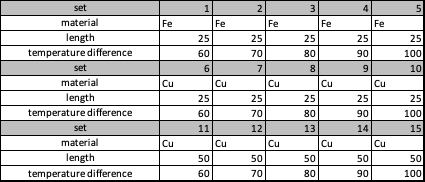
\includegraphics[width=0.8\textwidth]{Plan.png} %插入图片,[]中设置图片大小,{}中是图片文件名
\caption{Experiments Plan} %最终文档中希望显示的图片标题
\end{figure}






By controlling all the variables, we will conclude all hypotheses.


\subsection{Instruments}
\begin{enumerate}
	\item Arduino board: for data processing and recording, and for connecting the various sensors;
	\item TMP36GT9Z temperature sensor: used to detect the temperature data of each point and send it back to Arduino in real-time;
	\item Steel and copper metal rods: 10mm diameter, 250mm length, two each, as the object of the experiment, connected to both sides of the thermal conductivity of the copper sheet for measurement;
	\item Thermally conductive copper sheet: used to connect the heat source (hot water and ice water mixture) with the metal rod;
	\item Household thermostat heater: used as a heat source on the higher side of the temperature, which can be maintained at the set temperature.
\end{enumerate}






Our experiment will use Arduino UNO as a data collecting tool. It possesses 6 simulation signal input ports, so we can install 6 sensors on our metal rod isometrically. Arduino will be connected to our computer and upload temperature data measured by sensors at the frequency we set up.


In our experiments, we will use 10mm*250mm metal rods made of copper and steel with high thermal conductivity to make the experimental phenomena more visible.\cite{enwiki:1038093320} Both sides of the metal rod will be polished and connected to a copper sheet for its good quality at heat-conducting. Two copper sheets will be placed into constant temperature water and each side maintains a certain temperature difference. The temperature sensors will be mounted on 1/2, 1/4, 3/4, 1/8 and metal sheets, which will ensure the maximum application of the measured data.


In the experiment, we will carry out the circuit and equipment assembly according to the advance plan. In the experiment, we will stick the temperature sensing on the metal rod and fix the metal with rubber bands, etc., and preheat the heat source and the metal piece first, until the sensor on the metal piece shows that it reaches the required temperature and remains unchanged for a long time, and install the metal rod between it. Start the experiment and start the data acquisition program. The experiment will be carried out until the temperature indication is stable for a long time (i.e. the metal enters a steady-state) and then ends.







\begin{figure}[H] %H为当前位置,!htb为忽略美学标准,htbp为浮动图形
\centering %图片居中
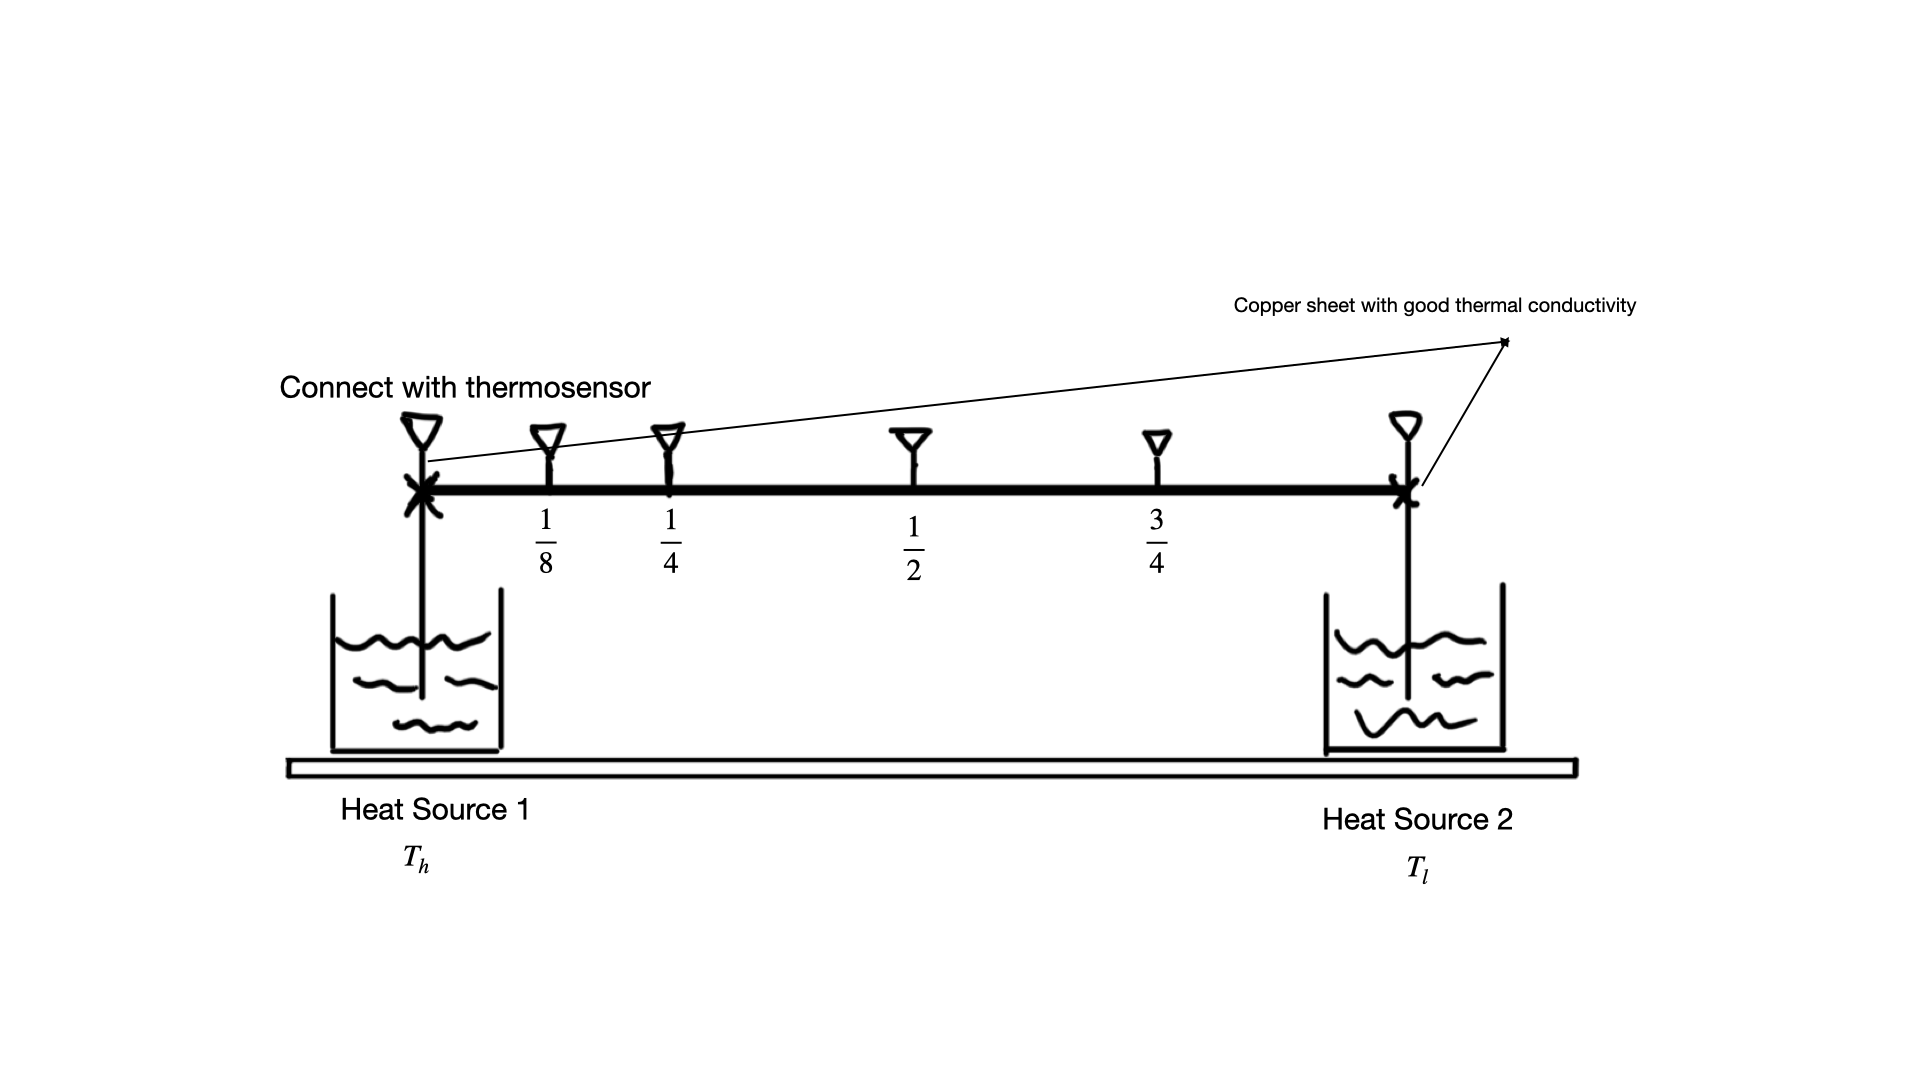
\includegraphics[width=1\textwidth]{插图带文字.001.png} %插入图片,[]中设置图片大小,{}中是图片文件名
\caption{Single Metal Stick} %最终文档中希望显示的图片标题
\end{figure}





\begin{figure}[H] %H为当前位置,!htb为忽略美学标准,htbp为浮动图形
\centering %图片居中
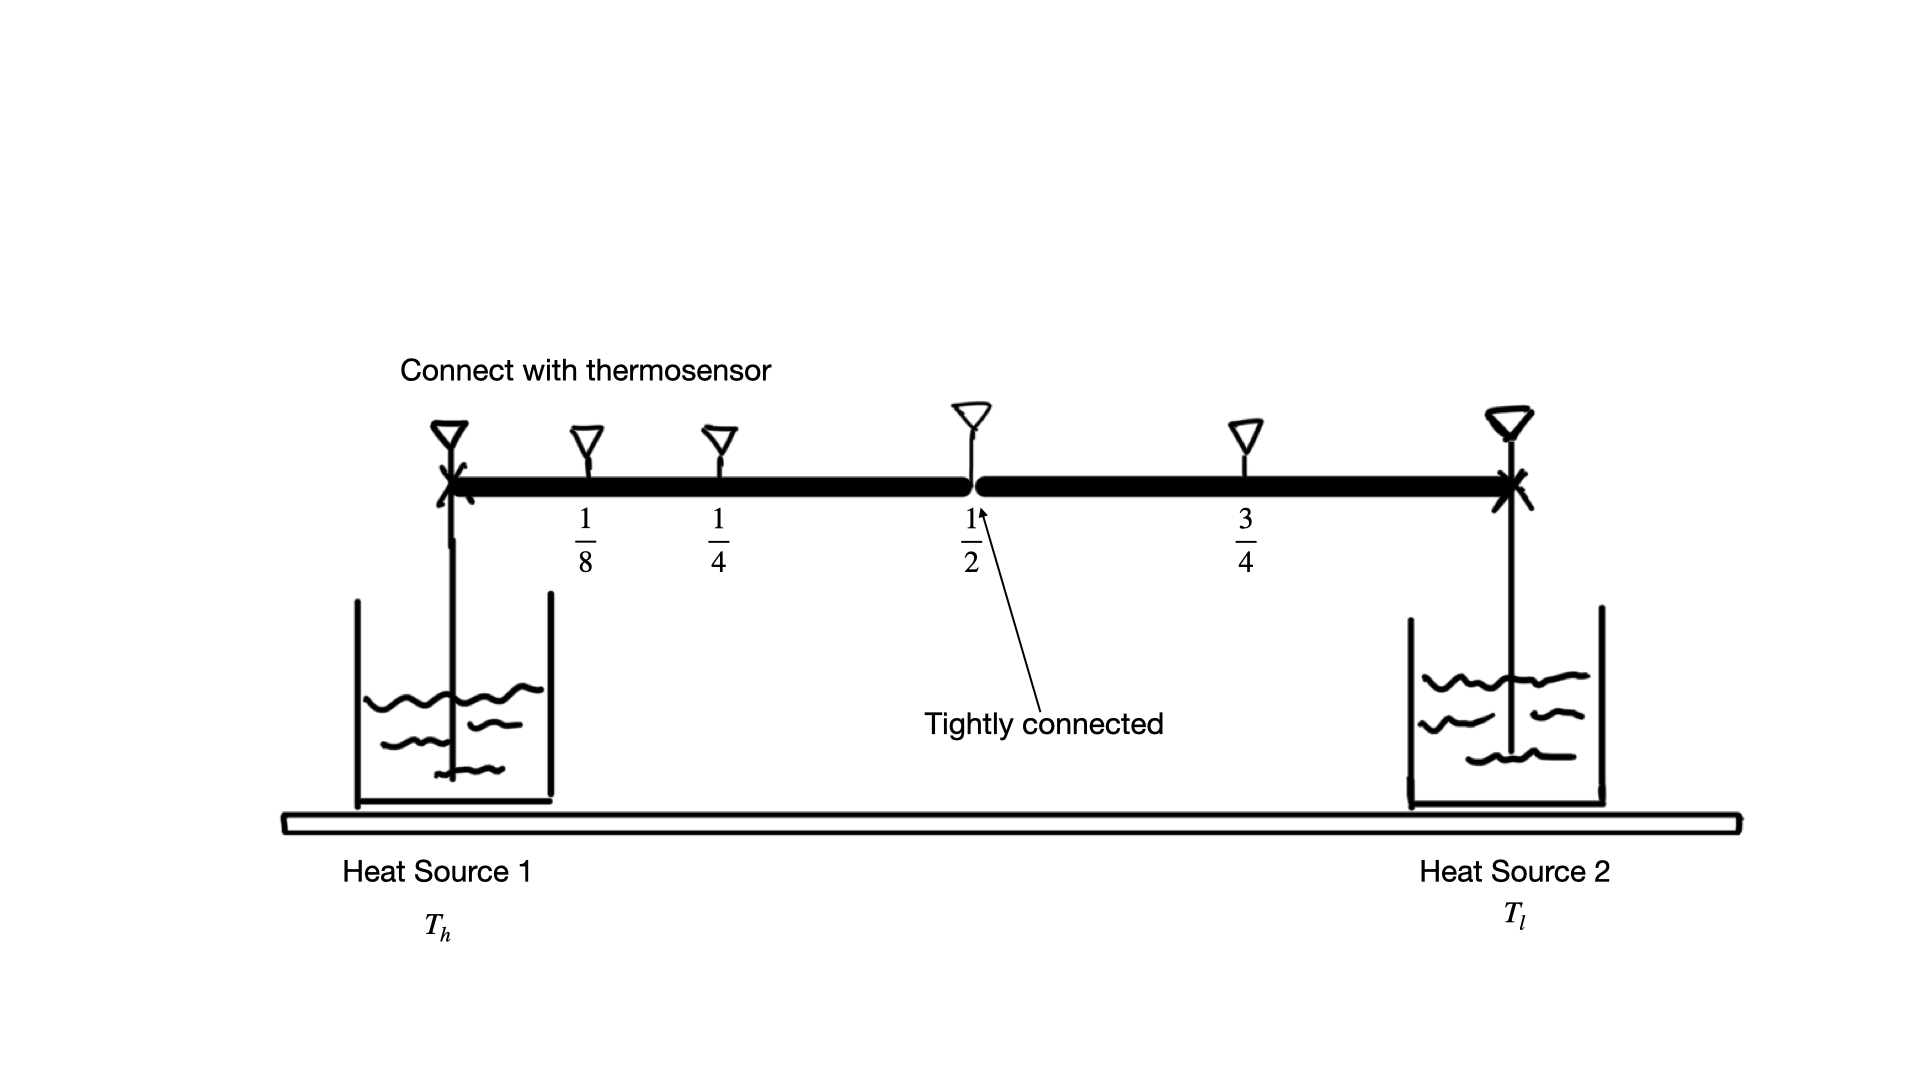
\includegraphics[width=0.8\textwidth]{插图带文字.002.png} %插入图片,[]中设置图片大小,{}中是图片文件名
\caption{Double Metal Stick} %最终文档中希望显示的图片标题
\end{figure}












\subsection{Data collecting}


In the experiment, we use Arduino and temperature sensors to collect data and send it back to a computer in real-time and record the time. Each experiment will be conducted 3 times, and when there is a large difference, the experiment will be redone. Since the experiment may be conducted in different locations, the data from each location will be processed separately, in the same way, to ensure that the experiment will not be interfered with by climatic factors.


The experiment started after the metal rod and the copper heat-conducting sheet were completely pressed against each other and ended when the temperature at each point did not change for a long time.




\subsection{Data analyzing}
With the time data collected and the corresponding temperature at each point, we will have the ability to plot the image of the temperature at each point with time and fit the image of the temperature at the same time point with the position. By taking the average slope as well as the maximum slope of the former and comparing it horizontally among the experimental groups, we will be able to draw the relationship between it and other factors and judge the hypothesis; by the latter with the change of time, the temperature change of the metal can be studied more deeply and more conclusions will be obtained.


For our experiment will be simulated on COMSOL with the whole process, we will get high-accuracy theoretical data, and these data can help us to do error analysis. After we sort out factors that might affect our experimental results, we can improve our experiment.


\begin{figure}[H] %H为当前位置,!htb为忽略美学标准,htbp为浮动图形
\centering %图片居中
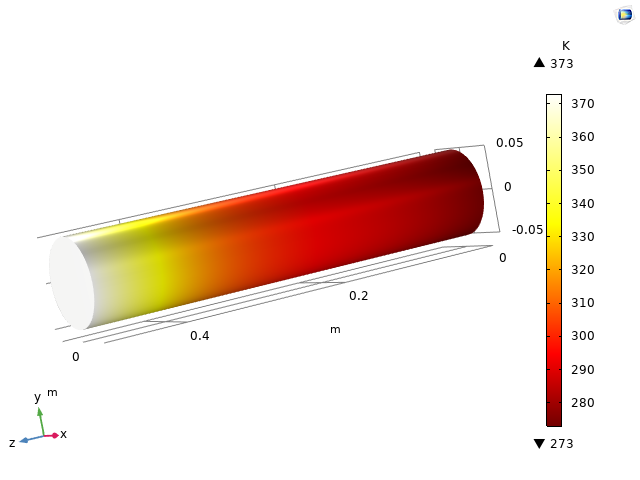
\includegraphics[width=0.7\textwidth]{COMSOL2.png} %插入图片,[]中设置图片大小,{}中是图片文件名
\caption{Budget Planning Chart} %最终文档中希望显示的图片标题
\end{figure}













\section{Milestone and Gantt Chart}

\paragraph{Milestone 1} Experimental set-up design completed
\paragraph{Milestone 2} Experimental circuit construction completed
\paragraph{Milestone 3} Experimental program and data processing program written
\paragraph{Milestone 4} Virtual COMSOL experiment completed
\paragraph{Milestone 5} Experimental investigation into the relationship between point temperature change and heat source temperature completed
\paragraph{Milestone 6} Experiment to investigate the relationship between temperature change at a point and length completed
\paragraph{Milestone 7} Experimental investigation into the relationship between point temperature change and point location completed
\paragraph{Milestone 8} complete a class 1 lab report
\paragraph{Milestone 9} Interim report submitted
\paragraph{Milestone 10} examine the relationship between the temperature at each point of the steady-state (especially the middle series) and the temperature of the heat source at each end
\paragraph{Milestone 11} check the temperature at each point of the steady-state (especially the middle series point) in relation to the order of the material connection Experiment completed
\paragraph{Milestone 12}Complete Data Analyse
\paragraph{Milestone 13} Submission of the overall experimental report
\paragraph{Milestone 14} Complete 2 types of experimental reports

\begin{figure}[H] %H为当前位置,!htb为忽略美学标准,htbp为浮动图形
\centering %图片居中
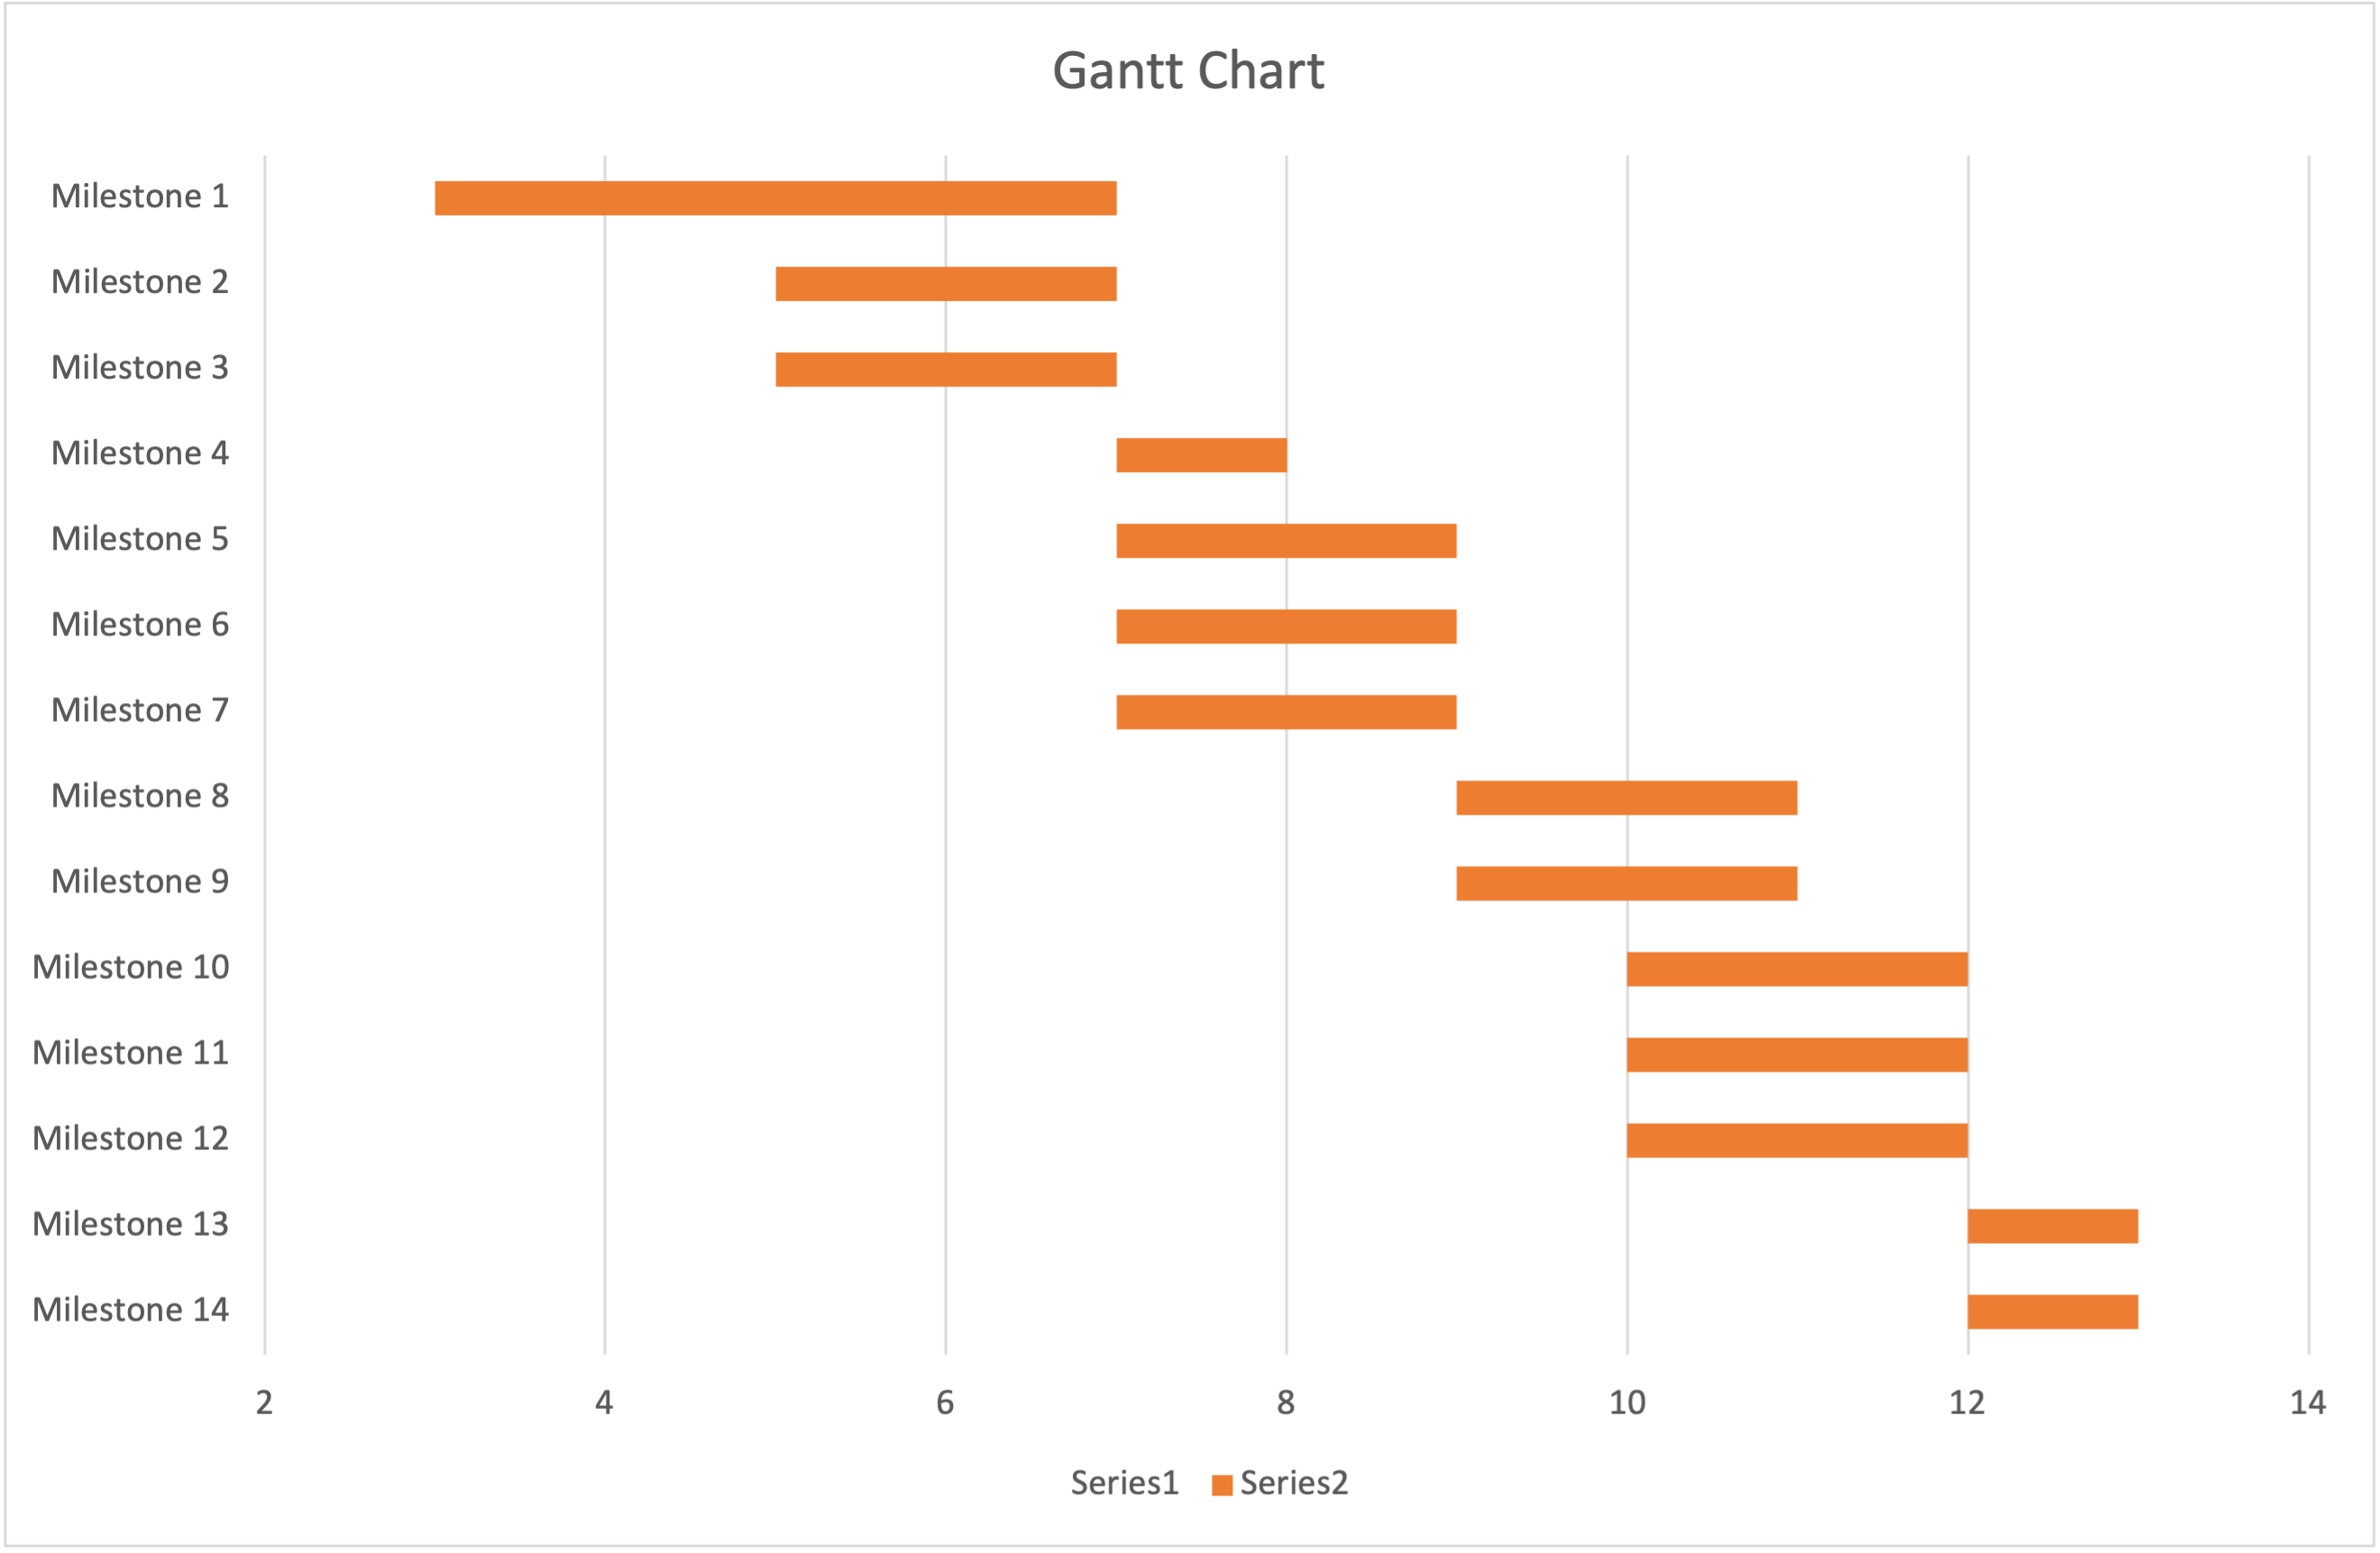
\includegraphics[width=0.9\textwidth]{Gantt.png} %插入图片,[]中设置图片大小,{}中是图片文件名
\caption{Gantt Chart} %最终文档中希望显示的图片标题
\end{figure}


\section{Budget Planning}

\paragraph{Unpredictable budget factor 1} Missing circuit parts due to damage or redesign of the circuit

\paragraph{Unpredictable budget factor 2} Unavailability due to damage, re-purchase due to unsuitable size. Metal bar prices exceed expectations


\begin{figure}[H] %H为当前位置,!htb为忽略美学标准,htbp为浮动图形
\centering %图片居中
\includegraphics[width=0.9\textwidth]{budget.png} %插入图片,[]中设置图片大小,{}中是图片文件名
\caption{COMSOL-based non-stationary temperature conduction model for cylinders} %最终文档中希望显示的图片标题
\end{figure}





\bibliographystyle{plain}
\bibliography{ref} 


\begin{appendices}
\section{Relevant Chart}
The all EXCEL chart could be find: \href{https://git.io/JrY5m}{https://git.io/JrY5m}

\section{Screenshot of Equipment Offer}


\begin{figure}[H] %H为当前位置,!htb为忽略美学标准,htbp为浮动图形
\centering %图片居中
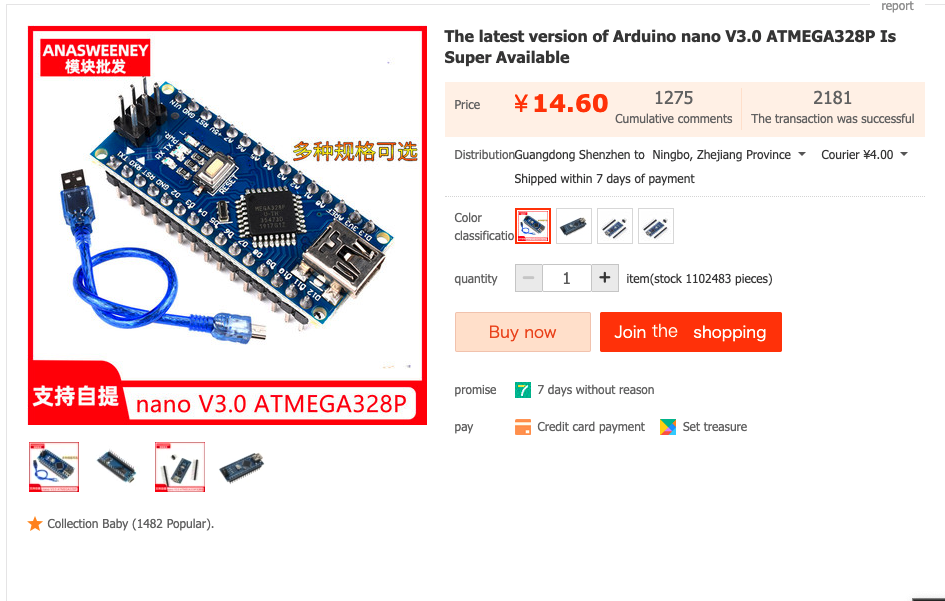
\includegraphics[width=0.5\textwidth]{NANO.png} %插入图片,[]中设置图片大小,{}中是图片文件名
\caption{Arduino Nano Board} %最终文档中希望显示的图片标题
\end{figure}

\begin{figure}[H] %H为当前位置,!htb为忽略美学标准,htbp为浮动图形
\centering %图片居中
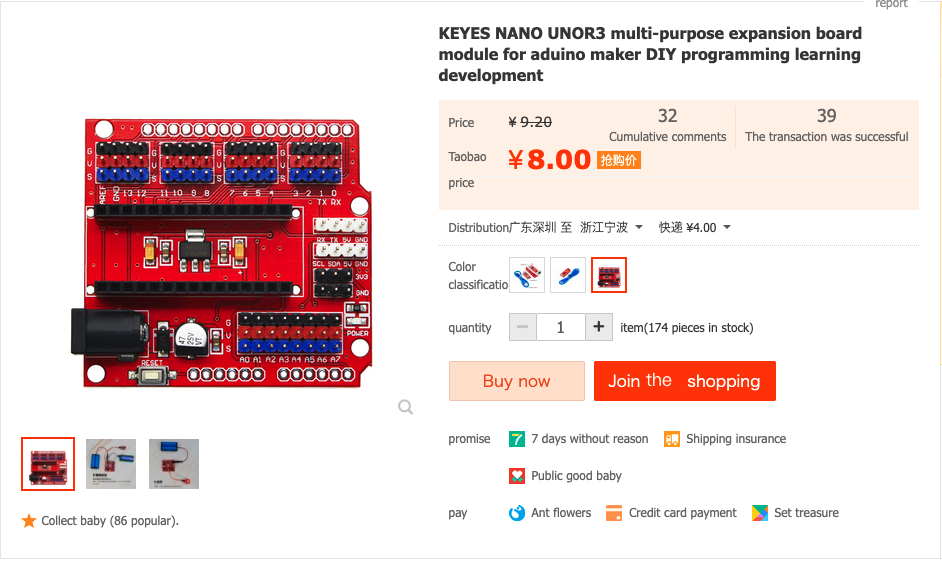
\includegraphics[width=0.5\textwidth]{Expansion.png} %插入图片,[]中设置图片大小,{}中是图片文件名
\caption{Arduino Nano Expansion Board} %最终文档中希望显示的图片标题
\end{figure}

\begin{figure}[H] %H为当前位置,!htb为忽略美学标准,htbp为浮动图形
\centering %图片居中
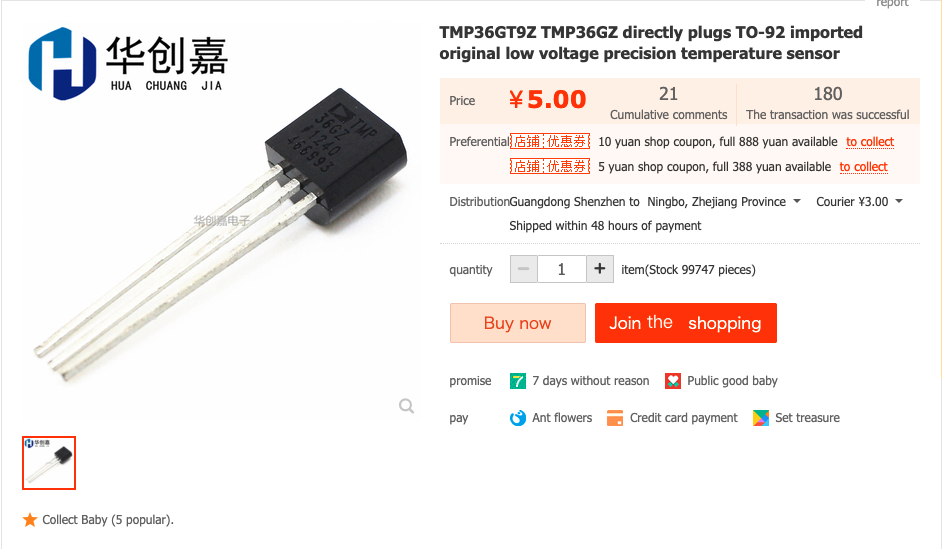
\includegraphics[width=0.5\textwidth]{tmp36.png} %插入图片,[]中设置图片大小,{}中是图片文件名
\caption{TMP36 Sensor} %最终文档中希望显示的图片标题
\end{figure}

\begin{figure}[H] %H为当前位置,!htb为忽略美学标准,htbp为浮动图形
\centering %图片居中
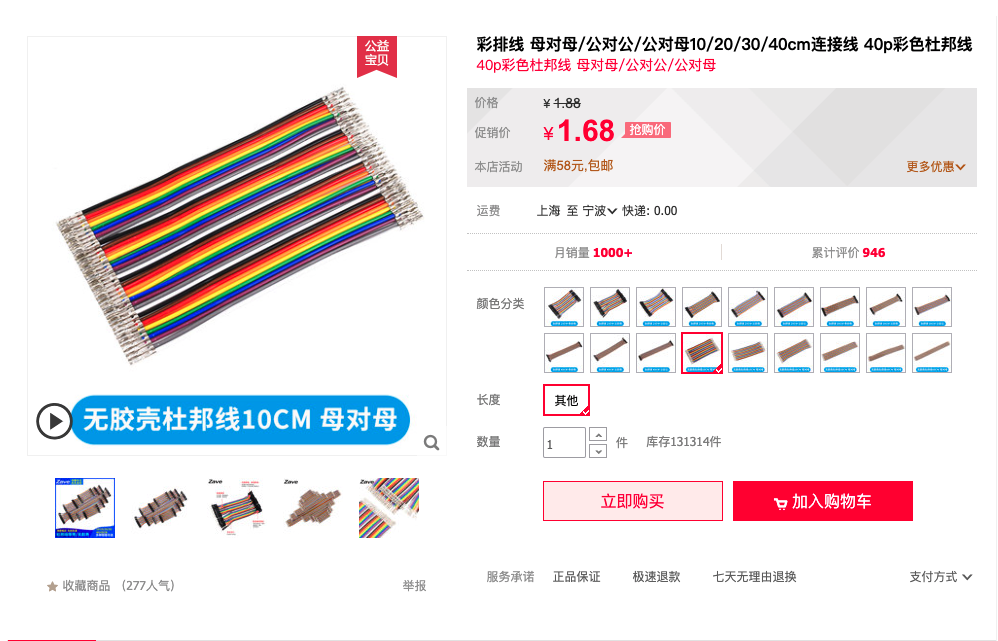
\includegraphics[width=0.5\textwidth]{line.png} %插入图片,[]中设置图片大小,{}中是图片文件名
\caption{Dupont Line} %最终文档中希望显示的图片标题
\end{figure}













\end{appendices}




























\end{document}

